\documentclass{beamer}
\usepackage{amsmath}
\usepackage[english]{babel} %set language; note: after changing this, you need to delete all auxiliary files to recompile
\usepackage[utf8]{inputenc} %define file encoding; latin1 is the other often used option
\usepackage{csquotes} % provides context sensitive quotation facilities
\usepackage{graphicx} %allows for inserting figures
\usepackage{booktabs} % for table formatting without vertical lines
\usepackage{textcomp} % allow for example using the Euro sign with \texteuro
\usepackage{stackengine}
\usepackage{wasysym}
\usepackage{tikzsymbols}
\usepackage{textcomp}
\usepackage{xcolor}
\usepackage[dvipsnames]{xcolor}
\usepackage{colortbl}
\usepackage{adjustbox}
\newcommand{\bubblethis}[2]{
        \tikz[remember picture,baseline]{\node[anchor=base,inner sep=0,outer sep=0]%
        (#1) {\underline{#1}};\node[overlay,cloud callout,callout relative pointer={(0.2cm,-0.7cm)},%
        aspect=2.5,fill=yellow!90] at ($(#1.north)+(-0.5cm,1.6cm)$) {#2};}%
    }%
\tikzset{face/.style={shape=circle,minimum size=4ex,shading=radial,outer sep=0pt,
        inner color=white!50!yellow,outer color= yellow!70!orange}}
%% Some commands to make the code easier
\newcommand{\emoticon}[1][]{%
  \node[face,#1] (emoticon) {};
  %% The eyes are fixed.
  \draw[fill=white] (-1ex,0ex) ..controls (-0.5ex,0.2ex)and(0.5ex,0.2ex)..
        (1ex,0.0ex) ..controls ( 1.5ex,1.5ex)and( 0.2ex,1.7ex)..
        (0ex,0.4ex) ..controls (-0.2ex,1.7ex)and(-1.5ex,1.5ex)..
        (-1ex,0ex)--cycle;}
\newcommand{\pupils}{
  %% standard pupils
  \fill[shift={(0.5ex,0.5ex)},rotate=80] 
       (0,0) ellipse (0.3ex and 0.15ex);
  \fill[shift={(-0.5ex,0.5ex)},rotate=100] 
       (0,0) ellipse (0.3ex and 0.15ex);}

\newcommand{\emoticonname}[1]{
  \node[below=1ex of emoticon,font=\footnotesize,
        minimum width=4cm]{#1};}
\usepackage{scalerel}
\usetikzlibrary{positioning}
\usetikzlibrary{decorations.pathreplacing}
\usepackage{xcolor,amssymb}
\newcommand\dangersignb[1][2ex]{%
  \scaleto{\stackengine{0.3pt}{\scalebox{1.1}[.9]{%
  \color{red}$\blacktriangle$}}{\tiny\bfseries !}{O}{c}{F}{F}{L}}{#1}%
}
\newcommand\dangersignw[1][2ex]{%
  \scaleto{\stackengine{0.3pt}{\scalebox{1.1}[.9]{%
  \color{red}$\blacktriangle$}}{\color{white}\tiny\bfseries !}{O}{c}{F}{F}{L}}{#1}%
}
\usepackage{fontawesome} % Social Icons
\usepackage{epstopdf} % allow embedding eps-figures
\usepackage{tikz} % allows drawing figures
\usepackage{amsmath,amssymb,amsthm} %advanced math facilities
\usepackage{lmodern} %uses font that support italic and bold at the same time
\usepackage{tikz}
\usepackage{tcolorbox}


\usefonttheme[onlymath]{serif} %set math font to serif ones

\definecolor{beamerblue}{rgb}{0.2,0.2,0.7} %define beamerblue color for later use

%%% defines highlight command to set text blue
\newcommand{\highlight}[1]{{\color{blue}{#1}}}


%%%%%%% commands defining backup slides so that frame numbering is correct

\newcommand{\backupbegin}{
   \newcounter{framenumberappendix}
   \setcounter{framenumberappendix}{\value{framenumber}}
}
\newcommand{\backupend}{
   \addtocounter{framenumberappendix}{-\value{framenumber}}
   \addtocounter{framenumber}{\value{framenumberappendix}}
}

%%%% end of defining backup slides

%Specify figure caption, see also http://tex.stackexchange.com/questions/155738/caption-package-not-working-with-beamer
\setbeamertemplate{caption}{\insertcaption} %redefines caption to remove label "Figure".
%\setbeamerfont{caption}{size=\scriptsize,shape=\itshape,series=\bfseries} %sets figure  caption bold and italic and makes it smaller


\newtcolorbox{boxA}{
    fontupper = \bf,
    boxrule = 1.5pt,
    colframe = black % frame color
}
\newtcolorbox{boxB}{
    boxrule = 1.5pt,
    colframe = blue!70!black,, % frame color
    colback = blue!7!white,
}

\usetheme{Boadilla}


\title[Economía I]{Economía I \vspace{4mm}
\\ Magistral 21: Mercado de Trabajo}
\date{}
\author[Franco Riottini]{Franco Riottini}
\vspace{0.4cm}
\institute[]{Universidad de San Andrés} 


\begin{document}

\begin{frame}
\titlepage
\centering

\includegraphics[scale=0.2]{../Figures/logoUDESA.jpg} 
\end{frame}

\begin{frame}{Mercado de Trabajo: conceptos clave}
    \vspace{0.3cm}
    \textbf{Oferta de trabajo: ¿Quiénes ofrecen trabajo?}
    \begin{itemize}
        \item Personas que buscan activamente empleo o están dispuestas a trabajar.
        \item La oferta puede medirse en cantidad de trabajadores o en horas totales ofrecidas.
    \end{itemize}

    \vspace{0.3cm}

    \textbf{Demanda de trabajo: ¿Quiénes demandan trabajo?}
    \begin{itemize}
        \item Empresas, organizaciones y particulares que desean contratar empleados o comprar horas de trabajo.
        \item Depende principalmente del valor que genera cada trabajador adicional para la producción (productividad marginal).
    \end{itemize}

    \vspace{0.3cm}

    \textbf{Salario:} es el precio del trabajo (puede ser nominal o real).
\end{frame}



\begin{frame}{Mercado de trabajo: demanda de trabajo}
    \footnotesize
    \textbf{La demanda de trabajo depende de:}
    \begin{itemize}
        \item \textbf{Salario} ($W$): las empresas comparan el salario con el valor que aporta un trabajador adicional.
        \item \textbf{Precio} ($P$): el precio de los bienes y servicios que producen las empresas.
        \item \textbf{Productividad marginal del trabajo}: cuánto valor adicional genera cada trabajador contratado.
    \end{itemize}

    \centering
    \begin{minipage}{0.48\textwidth}
        \begin{center}
            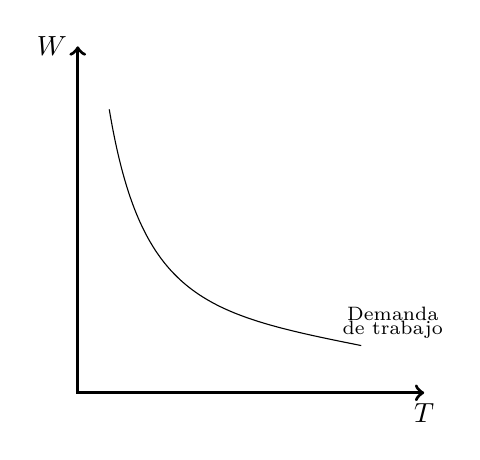
\begin{tikzpicture}[scale=0.4]
            \draw[very thick,<->] (0,11) node[left]{$W$}--(0,0)--(11,0) node[below]{$T$};
            \draw[thin] (1,9).. controls (2,3) and (4, 2.5) .. (9, 1.5);
            \node [] at (10,2.5) {\scriptsize Demanda};
            \node [] at (10,2) {\scriptsize de trabajo};
            \end{tikzpicture}
        \end{center}
    \end{minipage}
    \hfill
    \begin{minipage}{0.48\textwidth}
        \begin{center}
            \begin{figure}[H]
            \renewcommand{\figurename}{Figure}
            \begin{center}
            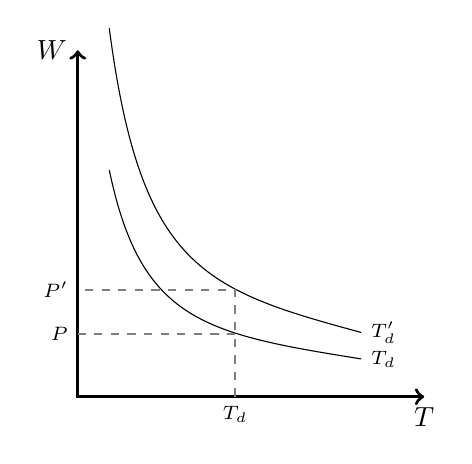
\begin{tikzpicture}[scale=0.4]
            \draw[very thick,<->] (0,11) node[left]{$W$}--(0,0)--(11,0) node[below]{$T$};
            \draw[thin] (1,7.2).. controls (2,2.4) and (4, 2) .. (9, 1.2) node [right] {\scriptsize $T_d$};
            \draw[thin] (1,11.7).. controls (2,4.08) and (4, 3.4) .. (9, 2.04) node [right] {\scriptsize$T_d'$}; 
            \draw[thick,gray,dashed](5,0)--(5,3.4)--(0,3.4);
            \draw[thick,gray,dashed](5,2)--(0,2);
            \node[left] at (0,2) {\scriptsize $P$};
            \node[left] at (0,3.4) {\scriptsize $P'$};
            \node[below] at (5,0) {\scriptsize $T_d$};
            \end{tikzpicture}
            \end{center}
            \end{figure}
        \end{center}
    \end{minipage}
\end{frame}

\begin{frame}{Mercado de trabajo: oferta de trabajo}
\small
\textbf{¿Cómo responde la oferta de trabajo ante cambios en el salario?}
\begin{enumerate}
\item \textbf{Shock transitorio (aumento temporal del salario):}
\begin{itemize}
    \item La oferta de trabajo \textbf{aumenta}.
    \item \textit{Efecto sustitución $>$ Efecto ingreso.}
    \begin{itemize}
        \item El tiempo libre se vuelve más caro $\Rightarrow$ se trabaja más.
        \item No hay tiempo suficiente para “sentirse más rico”.
    \end{itemize}
\end{itemize}

\item \textbf{Shock permanente (aumento sostenido del salario):}
\begin{itemize}
    \item La oferta de trabajo \textbf{no cambia significativamente}.
    \item \textit{Efecto sustitución $\simeq$ Efecto ingreso.}
    \begin{itemize}
        \item Se quiere trabajar más (sustitución).
        \item Pero también disfrutar más ocio (ingreso).
    \end{itemize}
\end{itemize}
\end{enumerate}
\textbf{Ejemplo histórico:}  
Desde la Edad Media, las horas trabajadas por día apenas han bajado (de 9 a 8 horas), a pesar de que los salarios reales aumentaron más de 6000\%. $\Rightarrow$ Elasticidad muy baja.
\end{frame}

\begin{frame}{Mercado de trabajo: oferta de trabajo}

\begin{columns}
\column{0.55\textwidth}

\textbf{Curvas de oferta de trabajo:}
    \small
    \begin{itemize}
        \item \textbf{LP (largo plazo):}  
        La oferta es \textbf{completamente inelástica} a partir de un salario de reserva \(\bar{W}\).
        
        \item \textbf{CP (corto plazo):}  
        Un aumento \textbf{transitorio} del salario genera más oferta de trabajo:  
        efecto sustitución \(>\) efecto ingreso.

        \item \textbf{Salario de reserva \(\bar{W}\):}  
        Mínimo salario aceptado para ofrecer trabajo.
    \end{itemize}
    \column{0.45\textwidth}
        \centering
        \includegraphics[width=\linewidth]{../Figures/C34.4.png}
    \end{columns}
\end{frame}

\begin{frame}{Mercado de trabajo: el equilibrio}
    \begin{columns}
    \column{0.55\textwidth}
    \footnotesize
    \begin{itemize}
        \item El salario de equilibrio (\(W^*\)) se alcanza cuando la \textbf{cantidad ofrecida} de trabajo coincide con la \textbf{cantidad demandada}.
        
        \item Si el salario es \textbf{mayor que \(W^*\)} (por ejemplo, \(W^{**}\)), las empresas quieren contratar menos trabajadores (\(T_d < T_o\)).

        \item Aparece entonces \textbf{desempleo involuntario}: personas dispuestas a trabajar al salario vigente, pero que no consiguen empleo.

        \item Para los \textbf{clásicos}, el salario baja hasta alcanzar \(W^*\) y eliminar el desempleo.

        \item Para los \textbf{keynesianos}, puede haber rigideces (ej. salarios mínimos, sindicatos, contratos) que impidan este ajuste.
    \end{itemize}

    \column{0.45\textwidth}
        \begin{center}
        \scriptsize
        \begin{figure}[H]
        \renewcommand{\figurename}{Figure}
        \begin{center}
        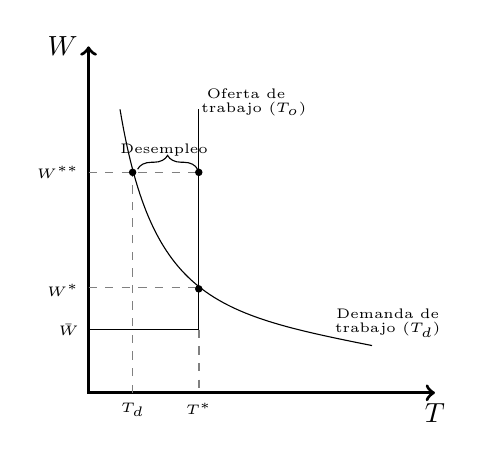
\begin{tikzpicture}[scale=0.4]
        \draw[very thick,<->] (0,11) node[left]{$W$}--(0,0)--(11,0) node[below]{$T$};
        \draw[thin] (1,9).. controls (2,3) and (4, 2.5) .. (9, 1.5);
        \node [] at (9.5,2.5) {\tiny Demanda de};
        \node [] at (9.5,2) {\tiny trabajo ($T_d$)};
        \draw[thin](3.5,2)--(3.5,9);
        \draw[thick, dashed, gray] (3.5,2)--(3.5,0);
        \node [] at (5,9.5) {\tiny Oferta de};
        \node [] at (5.25,9) {\tiny  trabajo ($T_o$)};
        \node [below] at (3.5,0) {\tiny  $T^*$};
        \node [left] at (0,3.25) {\tiny  $W^*$};
        \draw[thin, dashed,gray] (0,3.35)--(3.5,3.35);
        \node [left] at (0,7) {\tiny  $W^{**}$};
        \draw[thin, dashed,gray] (0,7)--(3.5,7);
        \draw (2.4,7.7) node[]{\tiny Desempleo};
        \draw[thin, dashed, gray] (1.4, 0)--(1.4,7);
        \node [below] at (1.4,0) {\tiny  $T_d$};
        \draw [thin,decorate,decoration={brace,amplitude=5pt},xshift=-4pt,yshift=0pt](1.7,7.1) -- (3.6,7.1);
        \node [left] at (0,2) {\tiny  $\bar{W}$}  ;
        \draw[thin] (0,2)--(3.5,2);
        \draw[fill](1.4,7) circle [radius =0.1];
        \draw[fill](3.5,7) circle [radius =0.1];
        \draw[fill](3.5,3.3) circle [radius =0.1];
        \end{tikzpicture}
        \end{center}
        \end{figure}
        \end{center}
    \end{columns}
\end{frame}

\begin{frame}{La visión de los Clásicos}
    \small
    \begin{itemize}
        \item Según esta visión el mercado de trabajo siempre está en equilibrio:
        \begin{itemize}
            \item Es decir que el $W^{*}$ es el de equilibrio
            \item Si no lo está, por alguna rigidez, surge un mercado informal que compensa
            \item De esta manera, el nivel de actividad es siempre el de pleno empleo
            \item Y la oferta agregada es vertical
        \end{itemize}
        \item ¿Qué explica el desempleo?
        \begin{itemize}
            \item Desempleo friccional: es el desempleo que existe incluso en equilibrio, derivado del tiempo que lleva emparejar trabajadores con empleos adecuados.
            \begin{itemize}
                \item Regulaciones laborales que dificultan contrataciones o despidos pueden alargar ese proceso.
                \item La búsqueda de empleo no es inmediata; los trabajadores evalúan ofertas, y las empresas seleccionan cuidadosamente.
                \item La existencia de seguros de desempleo puede reducir la urgencia de aceptar ofertas, prolongando la duración del desempleo friccional.
            \end{itemize}
            \item Salarios de reserva altos: si los trabajadores exigen salarios mínimos elevados por razones culturales, geográficas o familiares, puede haber menos empleos aceptables para ellos.
            \item Problemas de medición: puede clasificarse como desempleado a alguien que en realidad no está buscando activamente o que participa en actividades informales.
        \end{itemize}
    \end{itemize}
\end{frame}

\begin{frame}{La visión Keynesiana}
    \small
    El mercado de trabajo \textbf{no siempre} está en equilibrio:
    \begin{itemize}
        \item ¿Por qué puede el salario real permanecer fuera del equilibrio?
        \begin{itemize}
            \item Rigideces nominales: no se aceptan reducciones en el salario nominal, incluso si caen los precios.
            \item Sindicatos: salarios por encima del nivel de equilibrio
            \item Contratos de largo plazo: fijan salarios por períodos prolongados, impidiendo ajustes rápidos.
            \item Salarios de eficiencia: las empresas pagan salarios superiores al de mercado para incentivar esfuerzo o lealtad.
       \end{itemize}
    \end{itemize}
    \centering
    \includegraphics[scale=0.4]{../Figures/C34.7.png}
\end{frame}

\begin{frame}{Midiendo el desempleo}
    \begin{itemize}
        \item La EPH (Encuesta Permanente de Hogares) es una de las fuentes de datos más importantes para conocer la situación del mercado laboral en Argentina.
        
        \item Clasificamos a las personas según su relación con el mercado de trabajo:
        \begin{itemize}
            \item Población Económicamente Activa (PEA): personas que \textbf{trabajan} o \textbf{buscan activamente empleo}.
            \item Población Económicamente Inactiva: personas que no trabajan \textbf{ni buscan trabajo}, como estudiantes, jubilados, personas con tareas de cuidado, etc.
        \end{itemize}
        
        \item Los cambios en el desempleo pueden deberse no solo a despidos o contrataciones, sino también a movimientos entre la actividad y la inactividad.
        \begin{itemize}
            \item Ejemplo: una persona que estaba inactiva (no buscaba trabajo) comienza a buscar empleo y pasa a ser desempleada, aunque aún no haya sido contratada.
        \end{itemize}
    \end{itemize}
\end{frame}

\begin{frame}{Indicadores básicos del mercado laboral}
    \small
    \begin{itemize}
        \item \textit{Tasa de desempleo}: mide qué porcentaje de la PEA está desempleado.
        \[
        \text{Tasa de desempleo} = \frac{\text{Desempleados}}{\text{PEA}}
        \]
        
        \item \textit{Tasa de empleo}: indica qué parte de la población total está ocupada.
        \[
        \text{Tasa de empleo} = \frac{\text{Empleados}}{\text{Población}}
        \]
        
        \item \textit{Tasa de participación}: mide qué proporción de la población participa activamente del mercado laboral.
        \[
        \text{Tasa de participación} = \frac{\text{PEA}}{\text{Población}}
        \]
        
        \item \textbf{¡Cuidado!} La tasa de desempleo puede subir incluso si más personas consiguen empleo, si al mismo tiempo muchas más personas comienzan a buscar trabajo y se incorporan a la PEA.
    \end{itemize}

\end{frame}

\begin{frame}{¿Puede subir el desempleo aunque aumente el empleo?}
\small
Supongamos una población total de 100 personas.

\textbf{Situación inicial:}
\begin{itemize}
    \item Ocupados: 45 \quad Desempleados: 5 \quad Inactivos: 50
    \item PEA = \pause 45 + 5 = 50
    \item Tasa de desempleo = \pause 5 / 50 = 10\%
\end{itemize}
\textbf{Problema:}
\begin{itemize}
    \item 5 personas inactivas deciden buscar trabajo:
    \begin{itemize}
        \item 3 consiguen empleo $\rightarrow$ ocupados: \pause 48
        \item 2 no consiguen $\rightarrow$ desempleados: \pause 7
    \end{itemize}
    \item Nueva PEA = \pause 48 + 7 = 55
    \item Tasa de desempleo = \pause 7 / 55 $\approx$ 12{,}7\%
\end{itemize}
\textbf{Conclusión:}
\begin{itemize}
    \item Aumentó el empleo (\(+3\)) pero también el desempleo (\(+2\)).
    \item La tasa de desempleo subió, aunque haya más personas trabajando.
\end{itemize}
\end{frame}

\begin{frame}{La tasa de desempleo en Argentina durante el COVID}
    \centering
    \includegraphics[width=11cm]{../Figures/C34.15.png}
\end{frame}

\begin{frame}{El mercado de trabajo en la Argentina}
\centering\includegraphics[width=11cm]{../Figures/C34.17.png}
\end{frame}

\begin{frame}{El mercado de trabajo en la Argentina}
\centering\includegraphics[width=11cm]{../Figures/C34.18.png}
\end{frame}

\begin{frame}{El mercado de trabajo en la Argentina}
\centering\includegraphics[width=11cm]{../Figures/C34.19.png}
\end{frame}

\begin{frame}{¿Qué puede pasar con el desempleo en Argentina?}
    \small
    \textbf{Factores que podrían hacer que suba:}
    \begin{itemize}
        \item Estancamiento económico prolongado
        \item Reformas laborales sin incentivos a la contratación
        \item Ajustes fiscales o monetarios contractivos
        \item Caída del consumo interno
    \end{itemize}
    \vspace{0.15cm}
    \textbf{Factores que podrían hacer que baje:}
    \begin{itemize}
        \item Crecimiento sostenido con inversión productiva
        \item Políticas activas de empleo formal
        \item Mejoras en educación y capacitación laboral
    \end{itemize}
    \vspace{0.15cm}
    \textbf{Desafío estructural:}  
    Reducir el desempleo sin aumentar la informalidad. Mejorar la \textit{calidad} del empleo, no solo su cantidad.

    \vspace{0.15cm}
    \textbf{Interrogante:} ¿Y la IA? ¿Cómo afectará al mercado laboral en el futuro?
\end{frame}


\end{document}